\documentclass{article}

\usepackage{graphicx}
\usepackage{subfig}
\usepackage{listings}
\usepackage{color}
\usepackage{hyperref}
\usepackage{amsmath}
\usepackage{biblatex}

\definecolor{commentcolor}{rgb}{0,0.6,0}
\definecolor{stringliteralcolor}{rgb}{0.58,0,0.82}

\lstset{%
  language=java,
  backgroundcolor=\color{white},
  basicstyle=\footnotesize,
  breaklines=true,
  captionpos=b,
  commentstyle=\color{commentcolor},
  keywordstyle=\color{blue},
  stringstyle=\color{stringliteralcolor},
}

\title{PA 1: Bloom Filters}
\author{David Johnston}

\bibliography{refs}

\begin{document}
\maketitle

\begin{abstract}
\noindent
Bloom filters are a widely known and widely used probabilistic data structure.
In exchange for storing sets of elements very compactly, Bloom filters have
inherent but manageable false positive rates which arise from hashing
collisions. In this report, we first describe our implementation and evaluation
of two Bloom filter implementations, one using a deterministic hashing scheme
and the other using a random hashing scheme. We then used simulated data sets to
compare these Bloom filters' false positive rates. We found that the random
hashing scheme produced lower observed false positive rates. We additionally
used our deterministic Bloom filter to improve the performance of retrieval task
on a file-based key-value store with a given real-world data set. We then
performed a series of random queries on these two systems to measure performance
improvements. We found that the use of the Bloom filter design provided a 1.19x
speedup in overall query time and a mean per-query time speedup of 2.44x.
\end{abstract}

\section{Design and Implementation of \texttt{BloomFilterDet} and
         \texttt{BloomFilterRan}}

We implemented two bloom filters, \texttt{BloomFilterDet} and
\texttt{BloomFilterRan}. Both implement the \texttt{BloomFilter} interface,
which includes the methods specified in section 1.1 of the assignment document.

We use the class \texttt{LongBitSet} as the backing store (i.e. bit table) in
both bloom filters. This class was written by Mikhail Vorontsov and published
via \url{http://java-performance.info/bit-sets/}. It is essentially a wrapper
for the standard library's \texttt{BitSet} class to allow for indices of type
\texttt{long}. We used this data structure so that we could have a lazily
allocated but relatively efficient bit field with indices of type \texttt{long}.

The implementation of the bloom filter classes is quite simple. For this work,
the interesting challenges were all in the design of their hashing schemes.


\subsection{Designing \texttt{DeterministicHashFunctionFamily}: Turning One
            Hash into $k$ Hashes}

As the assignment document hints, an important aspect of implementing
\texttt{BloomFilterDet} is to convert a single 64-bit FNV hash function into a
set of $k$ deterministic hash functions, where $k$ is a function of the bits
per element, $b$.\footnote{
  Specifically, $k \in \{ \lfloor b \log(2) \rfloor, \lceil b \log(2) \rceil\}$,
  whichever minimizes the analytical false positive rate, $p$. However, in our
  current implementation we just set $k$ by rounding $b \log(2)$.
} Our solution, implemented within the \texttt{DeterministicHashFunctionFamily}
class, combines two strategies: slicing our hash into multiple bit fields and
making a family of hash functions via the double hashing formula.

We first hash the given string using the 64-bit FNV1 algorithm.\footnote{
  We used an implementation of the FNV1 algorithm written by Andrzej Bialecki
  and published via \url{http://www.getopt.org/}. This implementation is a
  rather direct Java port of \href{http://isthe.com/chongo/tech/comp/fnv/}{the
  reference implementation} written in C.
} This hash's results are then sliced in half to make a pair of 32-bit hashes
of our string. Thus, the lower 32-bits of FNV1 are used as one hash function,
$h_1$, and the upper 32-bits are used as another, $h_2$.

Let $m := nb$ define the number of bits in our table. For our bloom filter, we
need $k$ hash functions whose co-domain is the set of valid indices into this
table, that is, $[0..m)$.\footnote{Note that we limit $m$ to be values less than
$2^{32}$.} We follow the advice of Kirsch and Mitzenmacher \cite{kirsch2006less}
to turn this pair of hash functions into a family of $k$ hash functions: for
each $i \in [1..k]$,

$$g_i(x) = h_1(x) + i \cdot h_2(x) \mod m$$

The result is a family of $k$ hash functions which index into our table.


\subsection{Designing \texttt{RandomHashFunction}: Using a Universal Hashing Scheme}

Once again, the main challenge in implementing \texttt{BloomFilterRan} was
finding the right hashing scheme. We implemented the \texttt{RandomHashFunction}
class, whose instances represent a randomly generated hash function.

As specified in the assignment document, each of these random hash functions is
of the form $(ax + b \mod p) \mod m$.\footnote{
  We consulted Section 11.3.3 of \cite{cormen2009introduction} for details on
  valid choices of $a$, $b$, and $p$: $p$ is a prime larger than any potential
  value of $m$. $a$ and $b$ are uniformly randomly selected from $[1..p-1]$ and
  $[0..p-1]$, respectively.
} Notice that the domains of such hash functions are integerial, not strings of
arbitrary length. In our system, we needed to somehow encode Java
\texttt{String} as \texttt{int} without negatively our hashing behavior too
negatively. Dr. Aduri, recommended that we should use the
\texttt{String\#hashCode()} method to perform this conversion.


\section{Comparing Two Bloom Filters: \texttt{FalsePositives}}

With these implementations complete, we then started designing and implementing
the \texttt{FalsePositives} class, a simulated experiment measure false positive
rates under different conditions. In particular, we measure the false positive
rate as we vary three independent variables:

\begin{itemize}
  \item our Bloom filter implementation, $\texttt{f} \in
        \{ \texttt{BloomFilterDet}, \texttt{BloomFilterRan} \}$.
  \item set size, $n \in \{ 5000, 10000, 15000, 20000, 25000, 30000, 35000,
        40000, 45000, 50000 \}$.
  \item bits per element, $b \in \{ 4, 8, 12, 16 \}$).
\end{itemize}

For each of these combinations of $(f, n, b)$, we performed $N = 10000$ trials.
In each trial, the Bloom filter is populated with a set of randomly generated
strings.\footnote{
  Each random element is generated by the \texttt{FalsePositives\#randomString()}
  method. These strings are not uniformly random across all strings or even over
  a very common source of strings. These strings were generated by uniformly
  randomly generating \texttt{float} values in $[0, 1)$ and then converting
  these floats to their decimal \texttt{String} representation.
} Once the bloom filter is initialized with $n$ elements, we perform a certain
number of queries with values which were \textit{not} added to the bloom filter.
By counting the number of queries which are accepted, we are counting the number
of observed false positives. From this we can then compute this trial's $p^*$,
the observed false positive rate.

To select the number of queries per trial, we follow the example set by
\cite{kirsch2006less}: we perform $\lceil 10 / p \rceil$, where $p$ is the
analytically predicted false positive rate, given in the assignment document as
$p = (0.618)^b$. This way, as $p$ decreases and false positives become rarer, we
increase our number of queries and thus our number of chances to observe these
rarer false positives.\footnote{
  Whether this number of queries is \textit{sufficiently} large to get precise
  $p*$ estimates would require further analysis which we do not provide. There
  is a similar question as to whether $N = 10000$ trials is sufficiently large.
}

After all $N = 10000$ trials are performed, we take the mean of these observed
false positive rates. This gives us our mean false rate, $p*$ for some
combination of $f$, $n$, and $b$. In this way we compute our measured false
positive rate for all such combinations.

Figures ~\ref{fig:false_positives} and \ref{fig:normalized_false_positives}
summarize this data. Looking at this data, we make four brief observations:

\begin{itemize}
  \item Both bloom filters perform sub-optimally relative to their expected
        false positive rates (i.e. rates are always higher than predictions).
  \item \texttt{BloomFilterRet} appears to have somewhat better (i.e. lower)
        false positive rates than \texttt{BloomFilterDet}.
  \item False positive rates decrease as $b$ increases, as analytically
        predicted.
  \item False positive rates generally decrease as set size increases.
\end{itemize}

\begin{figure}[h]
  \makebox[\textwidth][c]{
    \subfloat[][$b=4$]{
      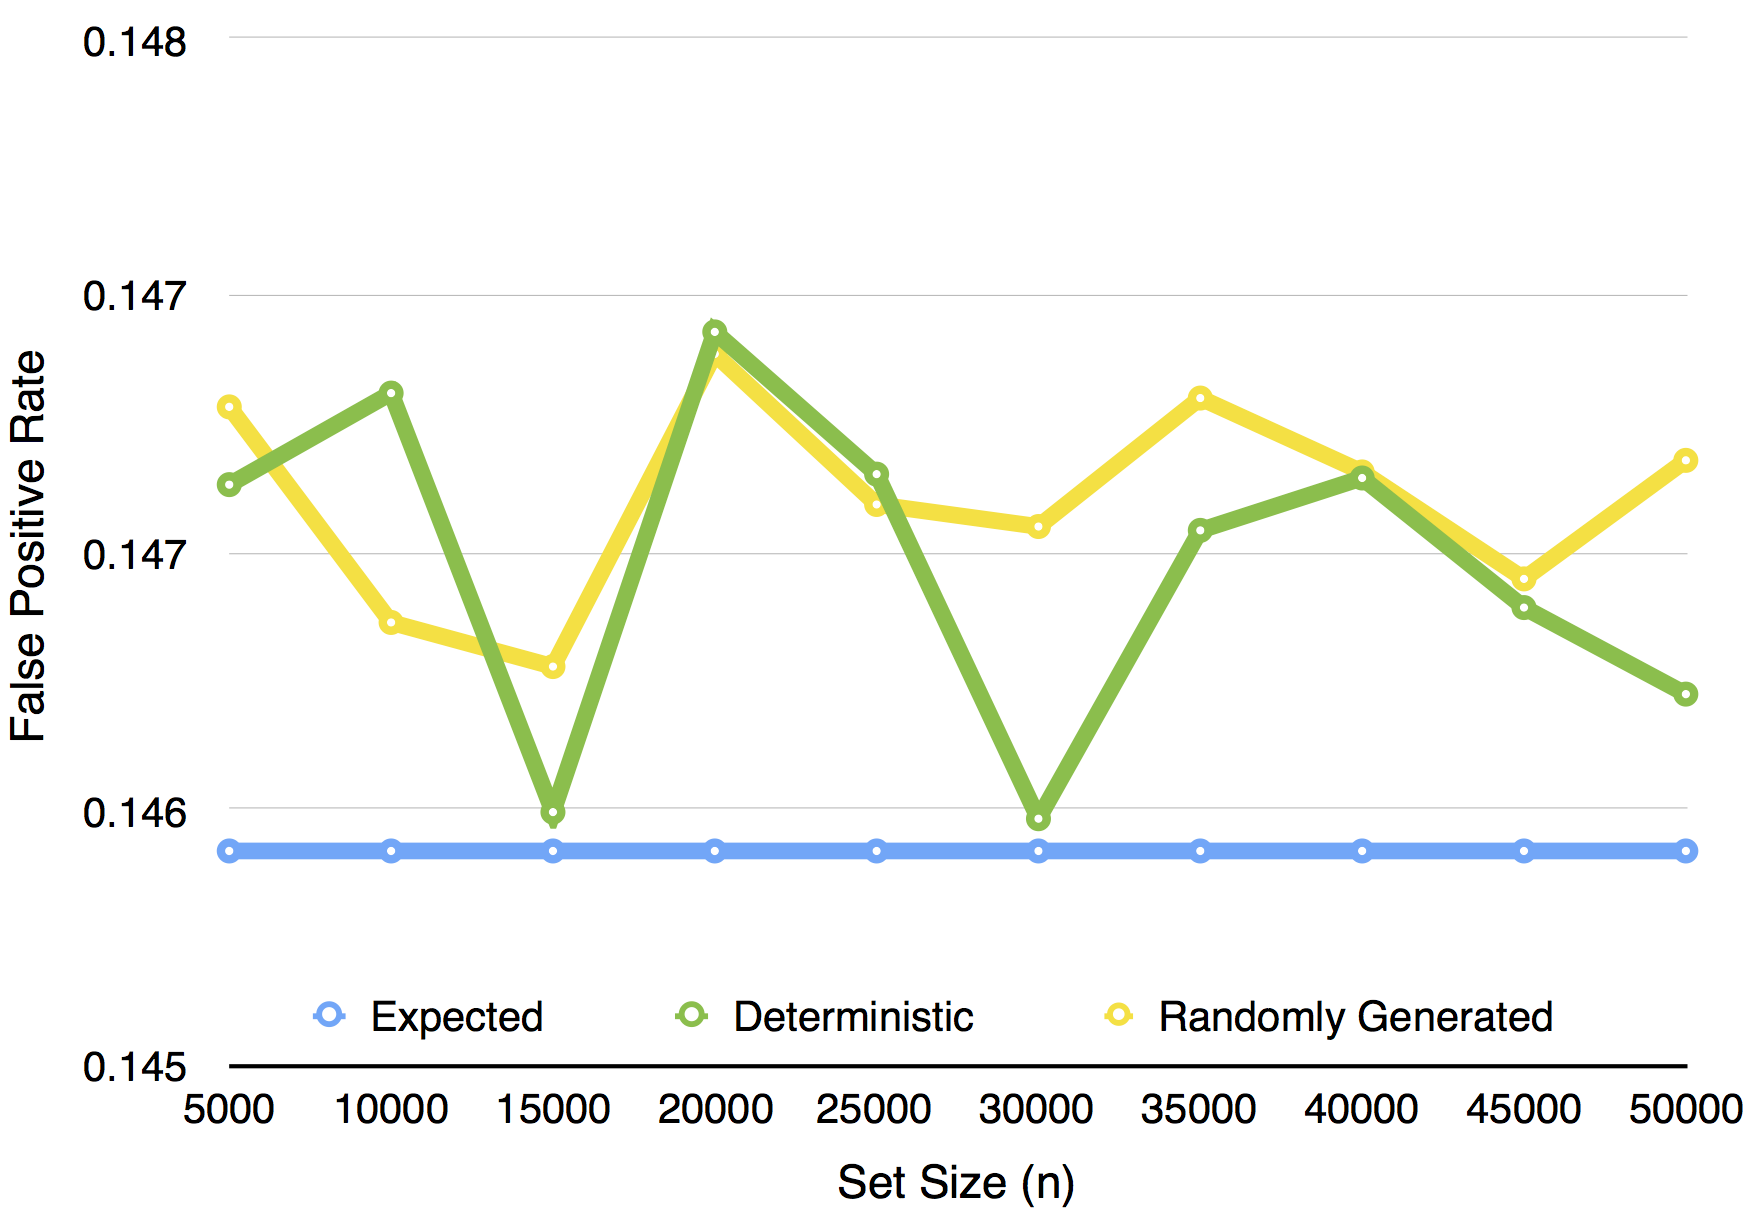
\includegraphics[width=0.65\textwidth]{figures/false_positives/b=4}
    }
    \subfloat[][$b=8$]{
      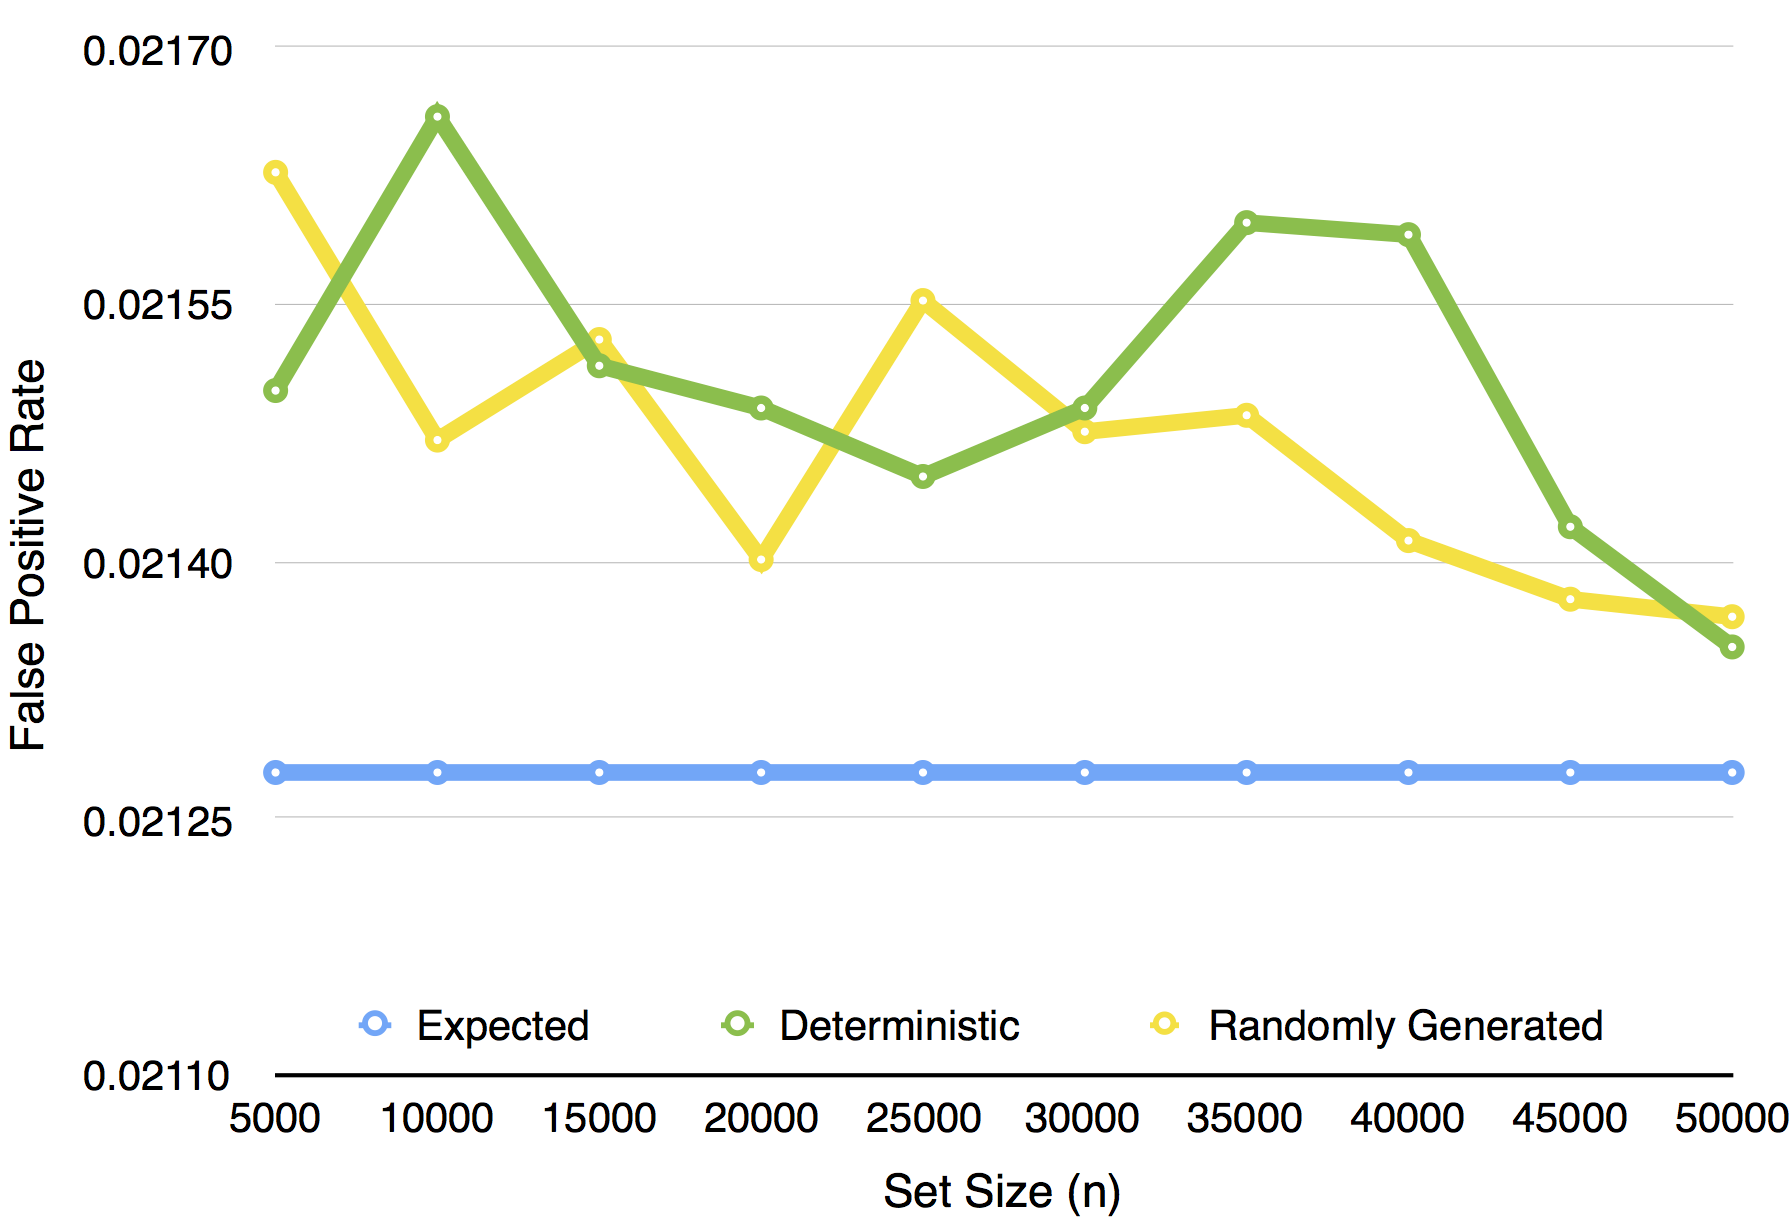
\includegraphics[width=0.65\textwidth]{figures/false_positives/b=8.png}
    }
  }

  \makebox[\textwidth][c]{
    \subfloat[][$b=12$]{
      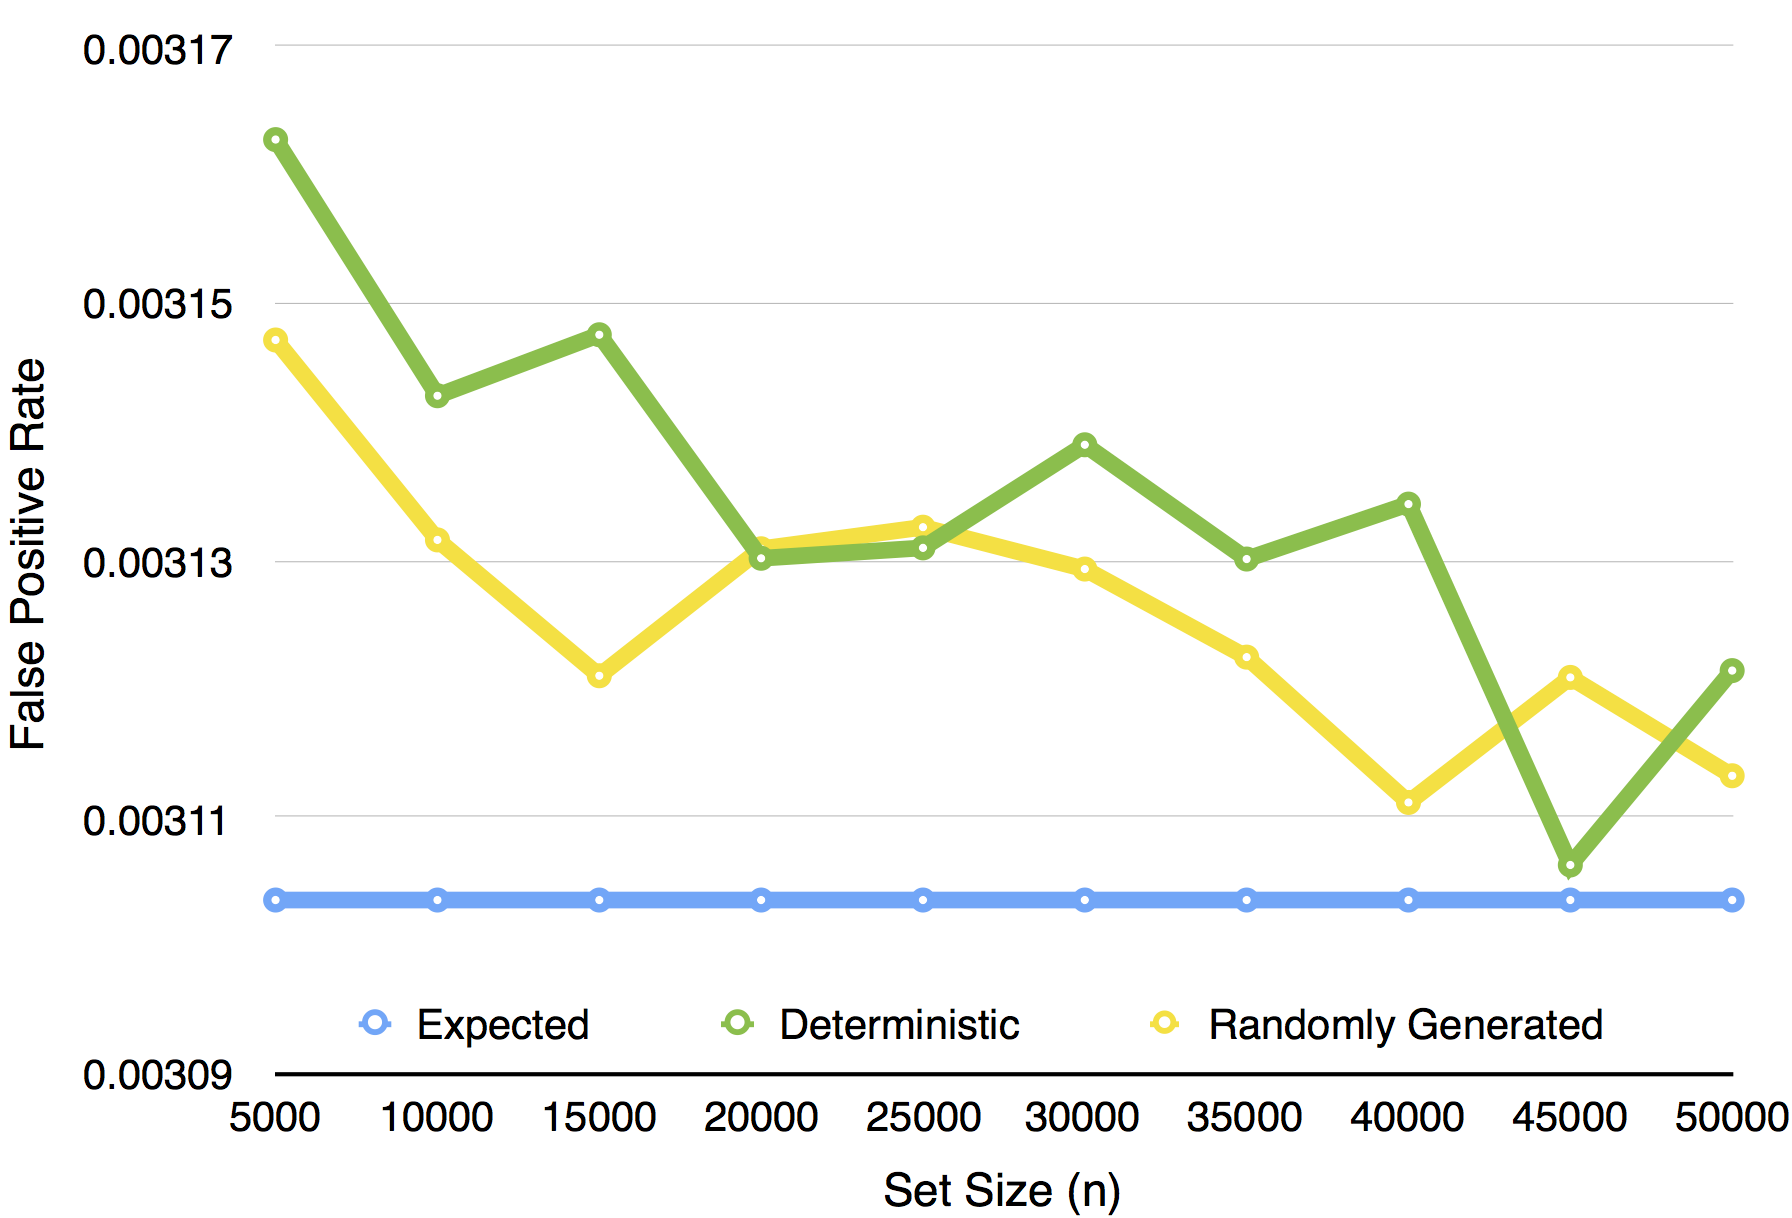
\includegraphics[width=0.65\textwidth]{figures/false_positives/b=12.png}
    }
    \subfloat[][$b=16$]{
      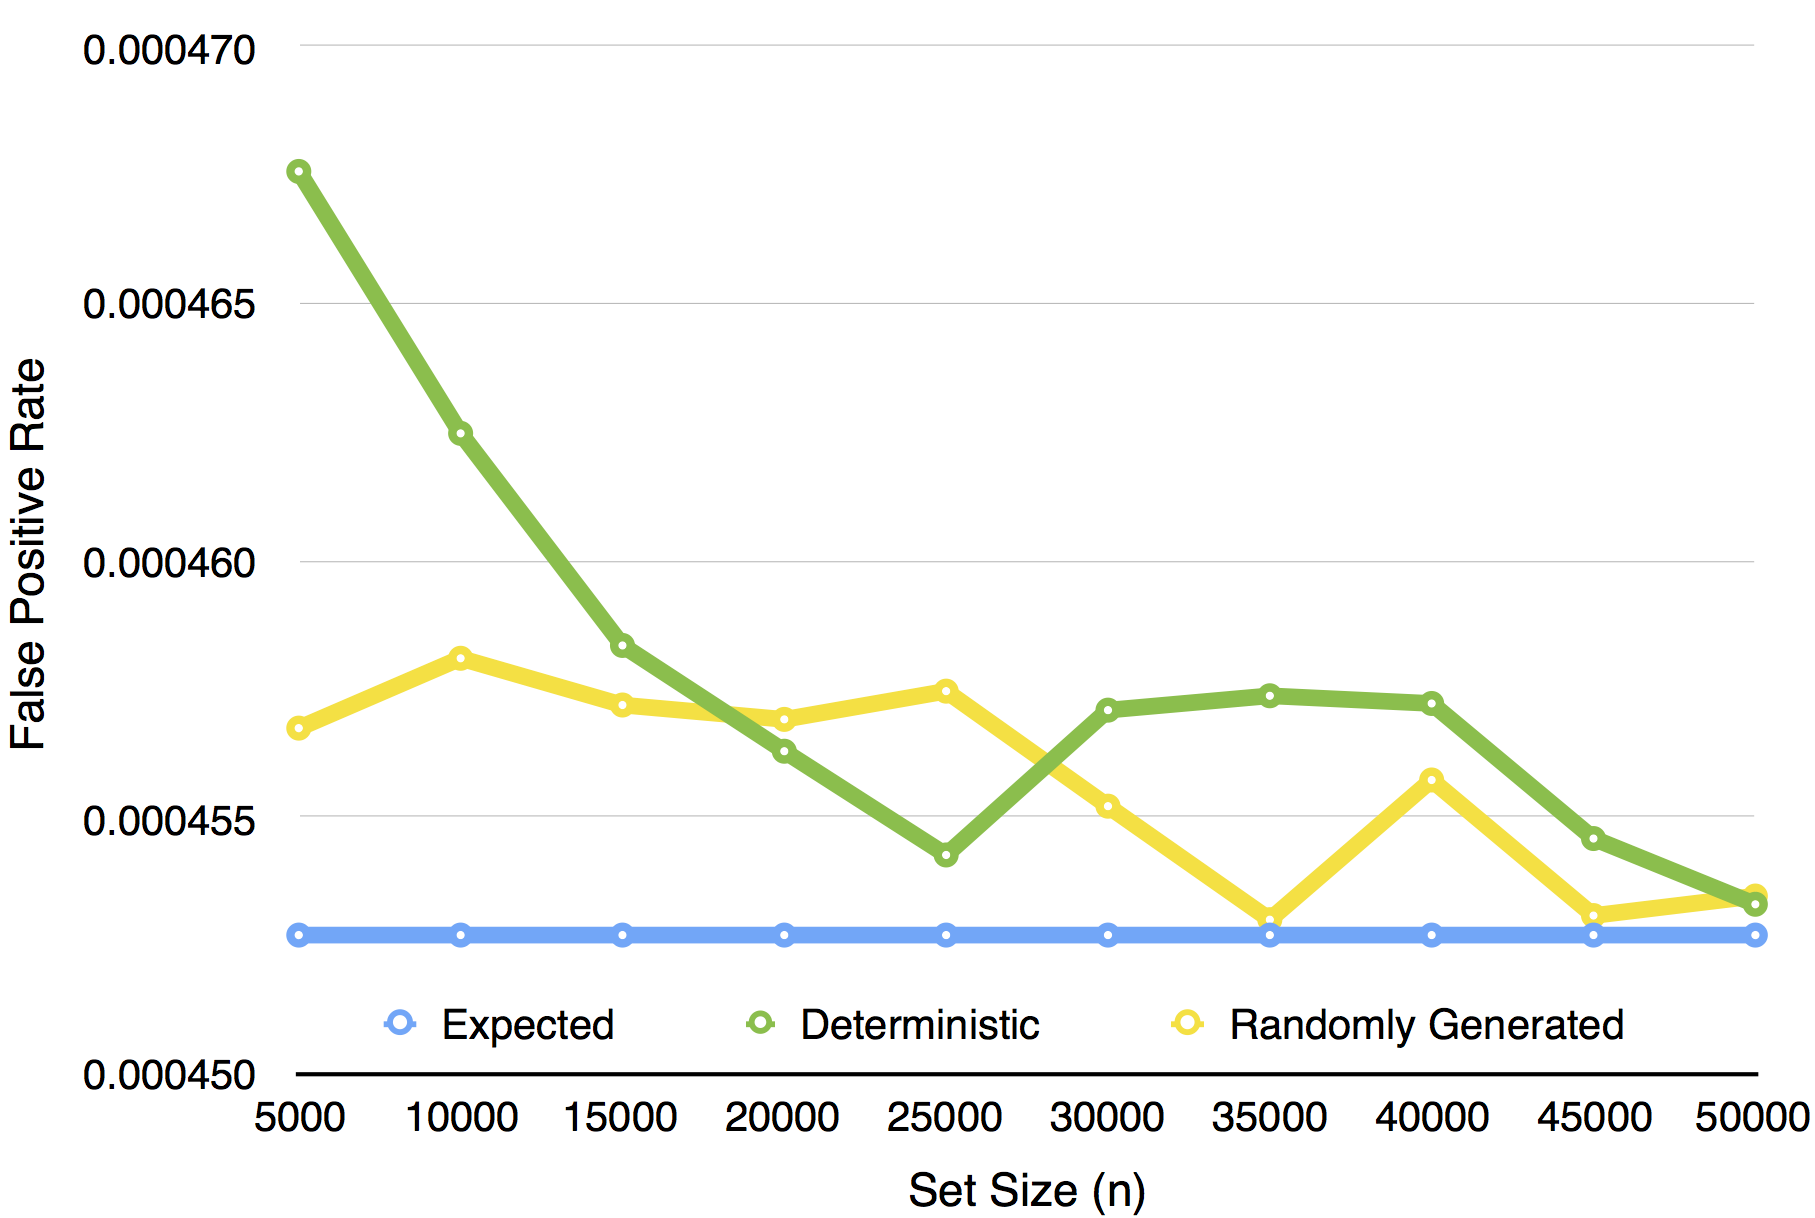
\includegraphics[width=0.65\textwidth]{figures/false_positives/b=16.png}
    }
  }

  \caption{Comparing expected and measured false positive rates of two Bloom
           filter implementations when varying set size ($n$) and
           bits per element ($b$). Notice that the vertical axes of these graphs
           use different scales: as $b$ increases the observed false positive
           rates decrease.}
  \label{fig:false_positives}
\end{figure}

\begin{figure}[h]
  \makebox[\textwidth][c]{
    \subfloat[][Deterministic]{
      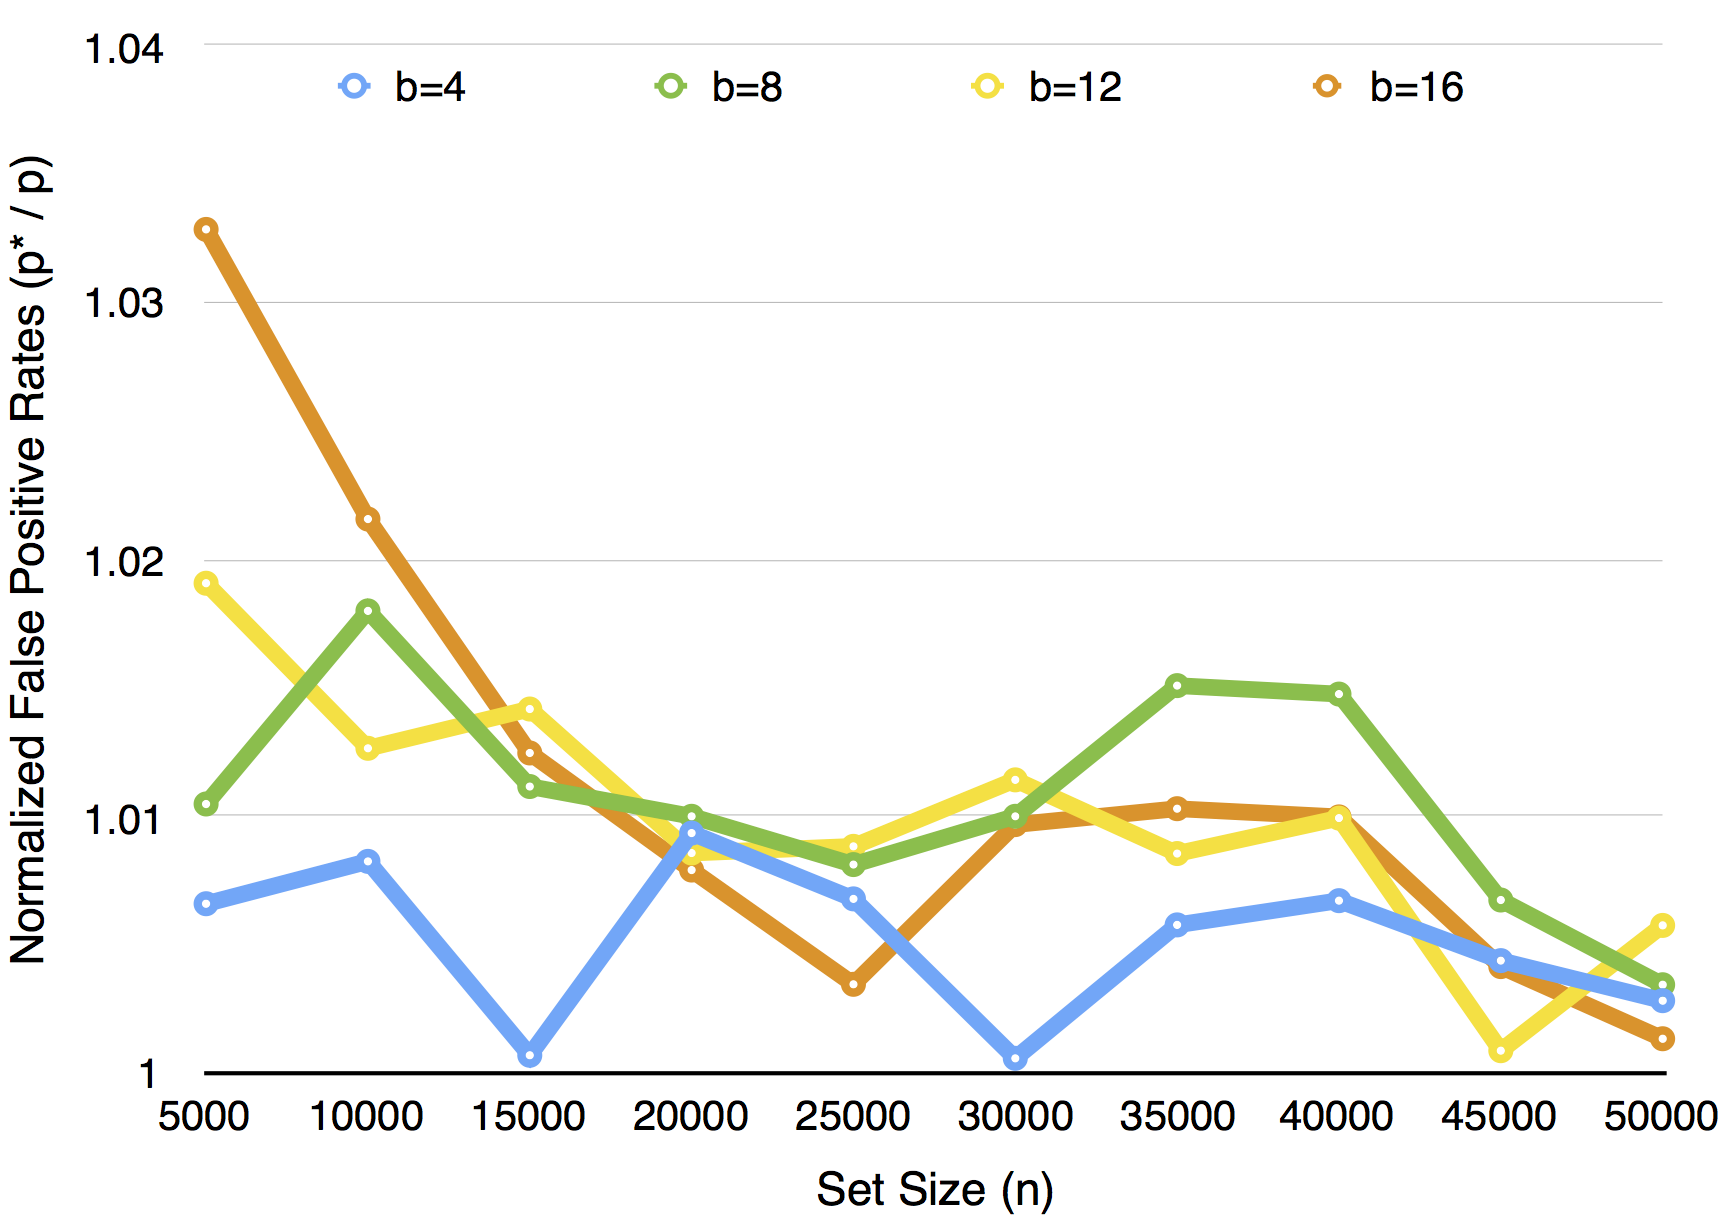
\includegraphics[width=0.65\textwidth]{figures/false_positives/normalized_deterministic.png}
    }
    \subfloat[][Randomly Generated]{
      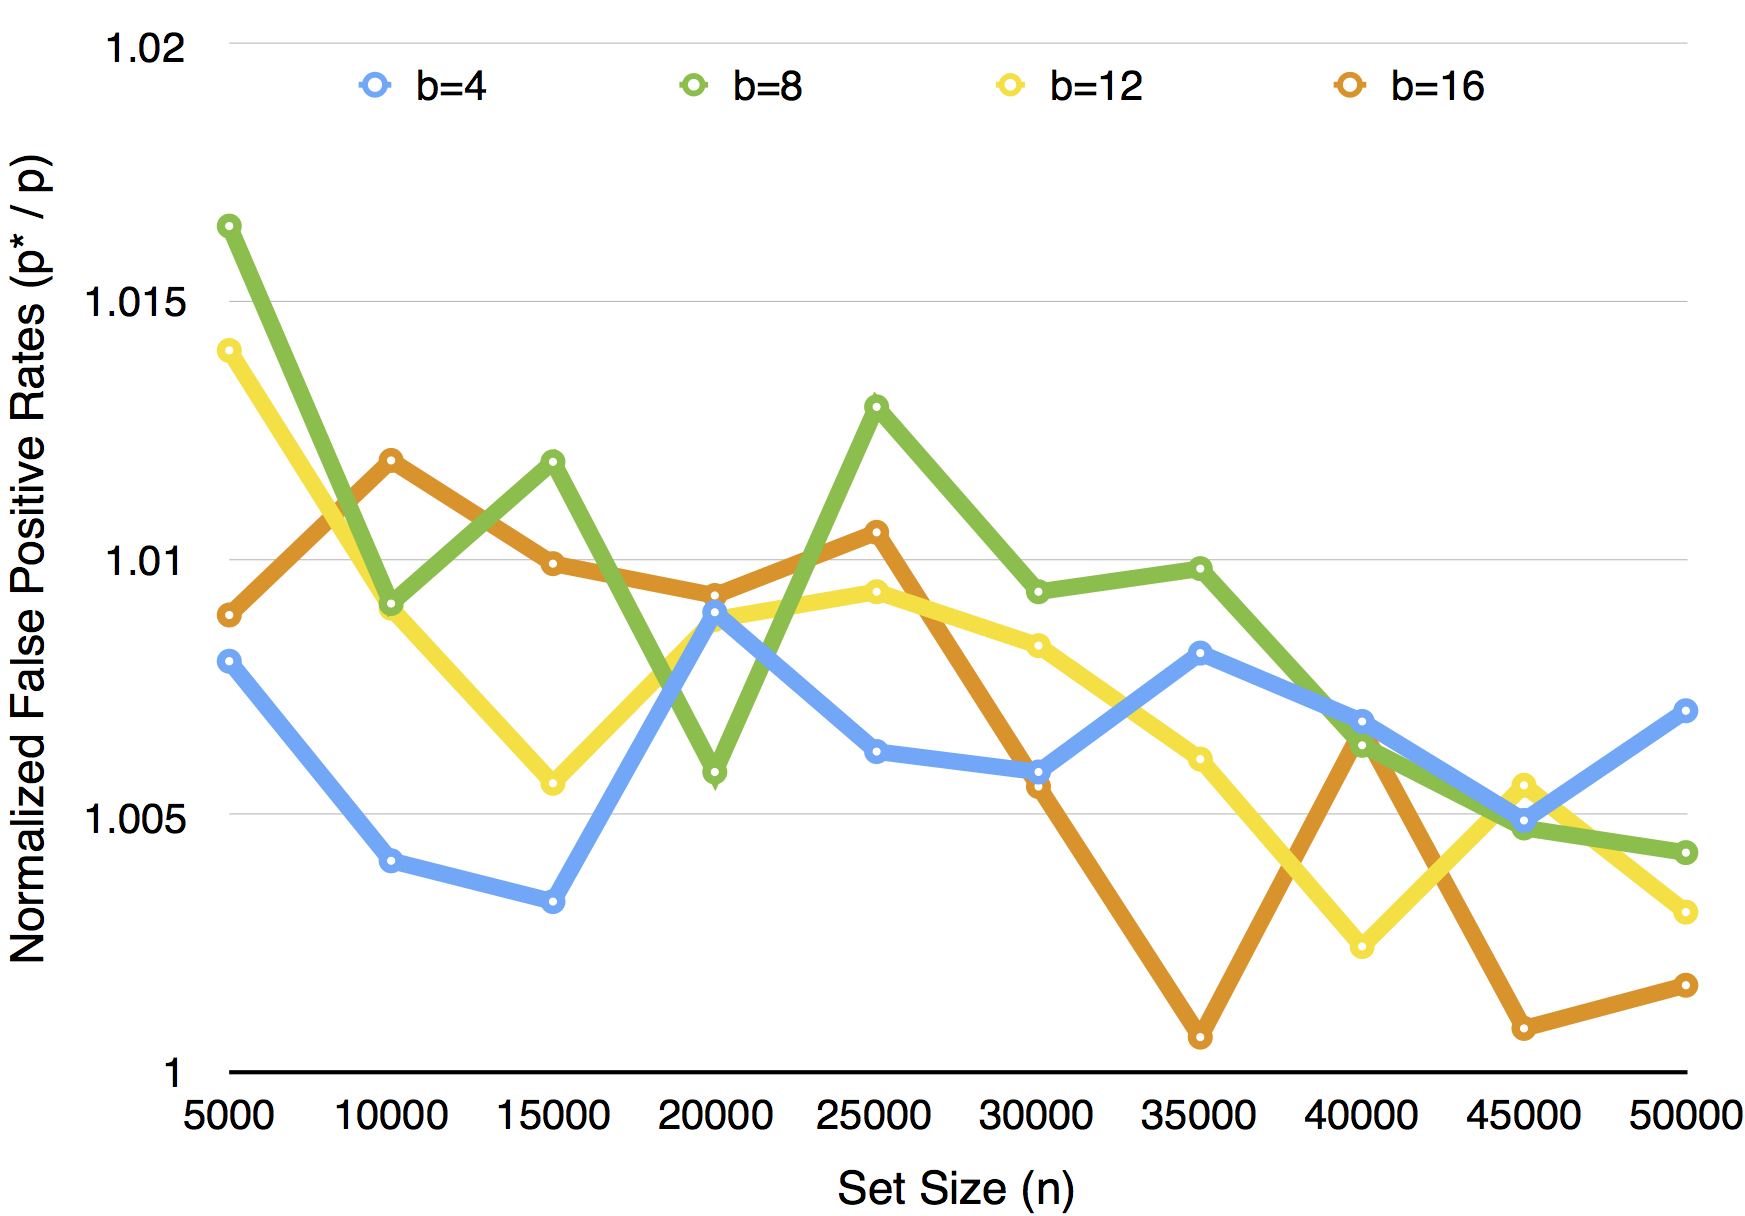
\includegraphics[width=0.65\textwidth]{figures/false_positives/normalized_random.png}
    }
  }
  \caption{Comparing normalized false positive rates when varying set size ($n$)
           and bits per element ($b$). Rates are normalized by dividing observed
           rates ($p*$) by the analytically expected rates ($p$). Note that each
           of the lines uses its own normalization factor: $p = 0.618^b$.}
  \label{fig:normalized_false_positives}
\end{figure}


\section{Two \texttt{Database} Implementers: \texttt{NaiveDifferential} and
         \texttt{BloomDifferential}}

We implemented \texttt{NaiveDifferential} and \texttt{BloomDifferential} as
directed. Both classes were made to implement a new interface,
\texttt{Database}, whose sole instance method is

\begin{lstlisting}
/**
 * Returns the value associated with this key, or else null
 * if this key was not found in the database.
 */
String retrieveRecord(String key);
\end{lstlisting}

The implementations of this method follow the specification document and are
thus straightforward. Note that \texttt{BloomFilterDet} (not
\texttt{BloomFilterRan}) was used in the implementation of
\texttt{BloomDifferential}.

The file-access and parsing functionality which is shared between the two
\texttt{Database} implementers was defined as a set of fairly trivial static
methods in \texttt{Database} itself:

\begin{lstlisting}
/**
 * Splits this line from a database file into a key-value pair.
 */
static Map.Entry<String, String> splitLine(String line) { ... }

/**
 * Searches the file indicated by the given path for an entry with
 * the given key. Each line of the file is parsed as a key-value
 * pair using the {@link #splitLine(String)} method.
 *
 * @returns An optional of the corresponding value if it was found,
 *          or {@link Optional#empty()} if no matching record was
 *          found.
 */
static Optional<String> retrieveRecordFrom(String key, Path path) {
    ...
}

/**
 * Scans the file indicated by the given path to count how many
 * lines it contains (or equivalently, the number of key-value
 * pairs which it contains).
 */
static int countLines(Path path) { ... }

/**
 * A helper method which scans {@link #DIFF_FILE} to see if it
 * contains the given key.
 */
static boolean isInDiffFile(String key) { ... }
\end{lstlisting}


\section{Designing \texttt{EmpiricalComparison} to Measure Speedup from the
         Bloom Filter}

The Bloom filter used in \texttt{BloomDifferential} is able to prevent many
potential accesses to \texttt{DiffFile.txt}, and we thus expect a noticeable
speedup over the \texttt{NaiveDifferential} implementation. As directed in the
assignment document, we designed \texttt{EmpiricalComparison} to simulate many
queries to both \texttt{NaiveDifferential} and \texttt{BloomDifferential} and to
measure this speedup.

We designed a run of \texttt{EmpiricalComparison} to behave in the following
way. We start by initializing both databases. We then uniformly randomly select
1264 keys from the \texttt{grams.txt} file. We then used the \texttt{java.time}
API to time the duration of a query on one of the databases and then the other.
The duration of each of these queries in milliseconds was recorded in CSV format
along with whether this key appears in \texttt{DiffFile.txt} and whether it
appears to be in the Bloom filter of the \texttt{BloomDifferential}.

We then used a Python-based Jupyter notebook using the Pandas library to perform
some basic data analysis on these durations. Overall query durations sum up to
5.15 hours. Of this time, more time was spent querying the
\texttt{NaiveDifferential} database, specifically, the
\texttt{BloomDifferential} implementation provided a 1.19x speedup.

When we look at individual queries, we see that mean \texttt{NaiveDifferential}
duration was 7.985 seconds, while that of \texttt{BloomDifferential} was 6.709
seconds. See Figure ~\ref{fig:query_duration_box_plot} for a comparison of the
two databases's duration distributions.

\begin{figure}[h]
  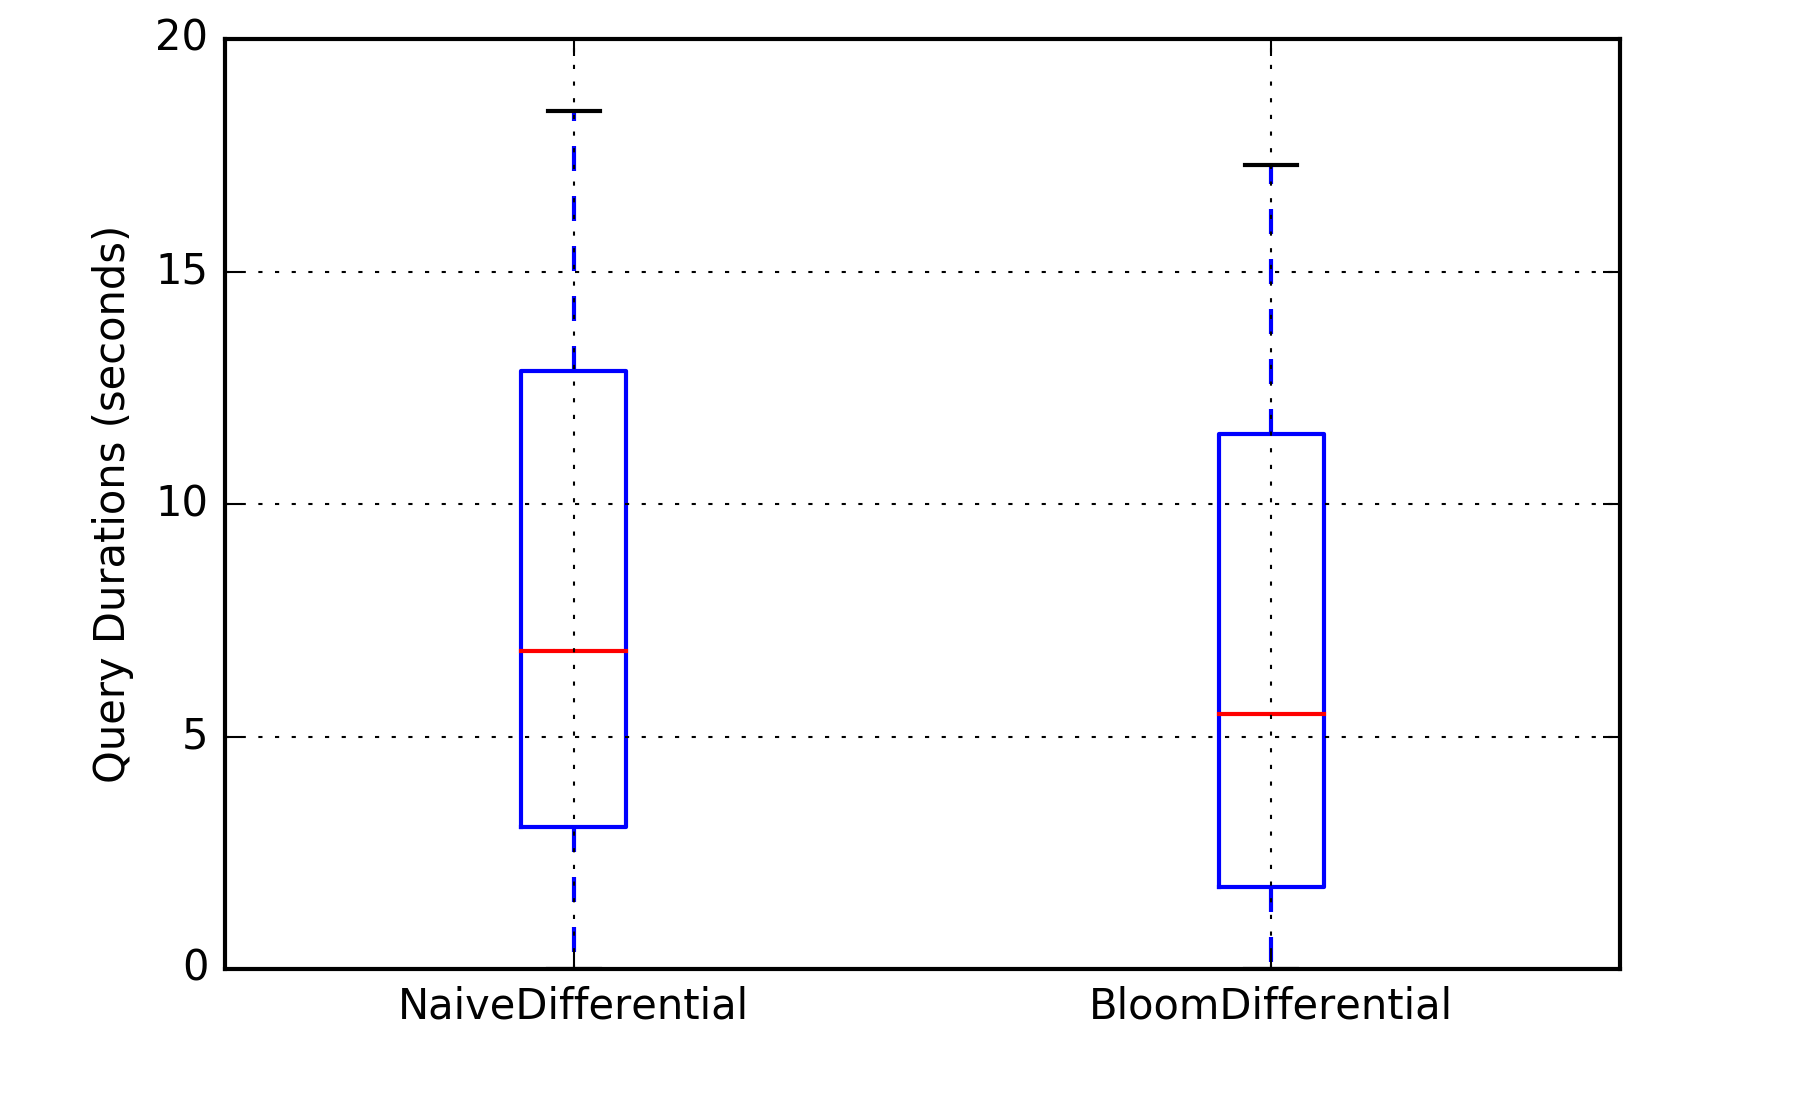
\includegraphics[width=\textwidth]{figures/empirical_comparison/query_duration_box_plot.png}
  \caption{Comparing query duration distributions of two database
           implementations.}
  \label{fig:query_duration_box_plot}
\end{figure}

When we compute the per-query speedup, we found the mean speedup to be 2.44x.
Looking at the box plot in Figure ~\ref{fig:query_speedup_box_plot}, we can see
that this distribution has a long tail upward, indicating that for speedup was
dramatic for some small proportion of queries. In fact, the max observed speedup
was 701.5x. The mean speedup was clearly quite influenced by this long tail, so
the median speedup, 1.234x, may be a better characterization of ``normal''
speedup than the mean speedup.

\begin{figure}[h]
  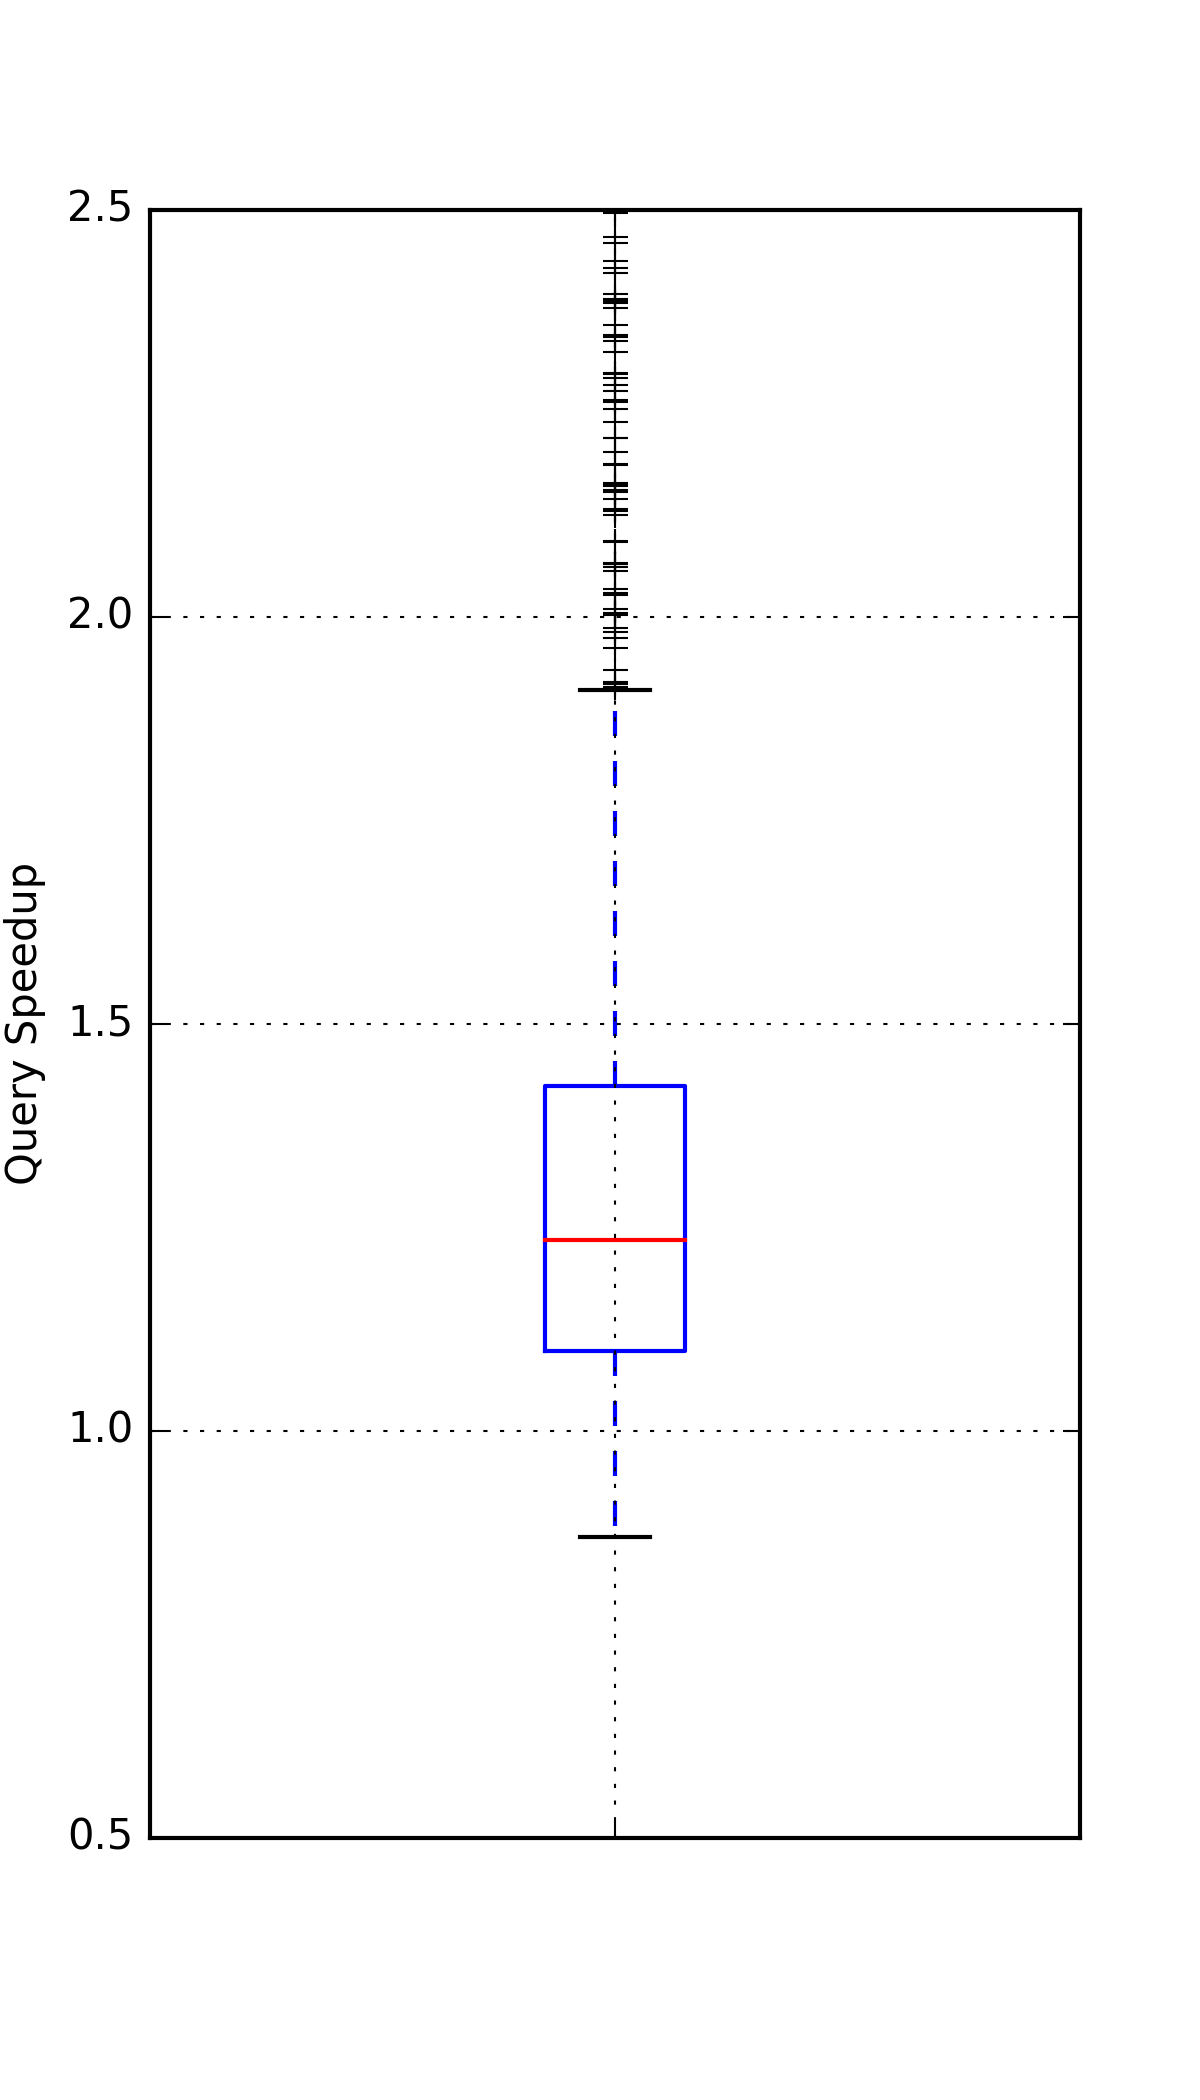
\includegraphics[width=\textwidth]{figures/empirical_comparison/query_speedup_box_plot.png}
  \caption{A distribution of per-query speedup values.}
  \label{fig:query_speedup_box_plot}
\end{figure}

\printbibliography

\end{document}
